\documentclass{fkssolpub}

\usepackage[czech]{babel}
\usepackage{fontspec}

\usepackage{fkssugar}
\usepackage{graphicx}
\usepackage{tikz}

\usetikzlibrary{angles, quotes}
 
\author{Ondřej Sedláček}
\school{Gymnázium Oty Pavla} 
\series{3}
\problem{4} 

\begin{document} 

Zdrojové soubory všech těchto úloh jsou přiloženy spolu s popisem.

\section{Úloha 1}

Výsledný graf funkce je tento:

\begin{figure}[h]
  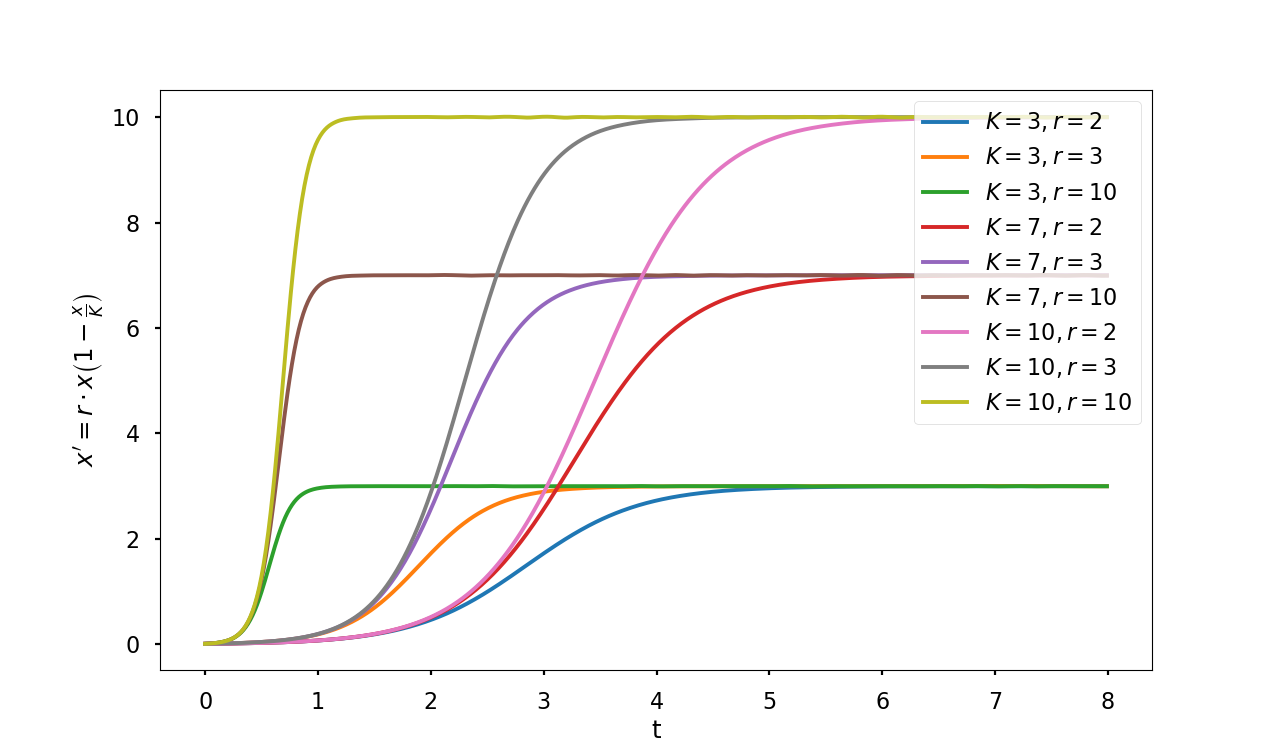
\includegraphics[width=0.8\textwidth]{Figure_1.png}
  \centering
\end{figure}

Pro ukázku jsem tam nevykresloval jen jednu funkci, ale několik funkcí s
rozdílnými parametry. Můžeme vypozorovat, že parametr $r$ určuje rychlost
růstu funkce. U parametru to vypadá, že parametr $K$ udává horní mez,
ale můžeme si všimnout především u funkce s parametry $K = 10, r = 10$,
že na konci, kde by měla být funkce konstantní, se funkce vlní. Poněvadž
jsem měl podezření, že se jedná o chybu (s velkou pravděpodobností chybě
čísel s plovoucí čárkou), spustil jsem to znova s počáteční hodnotou
rovno kapacitě $K$:

\begin{figure}[h]
  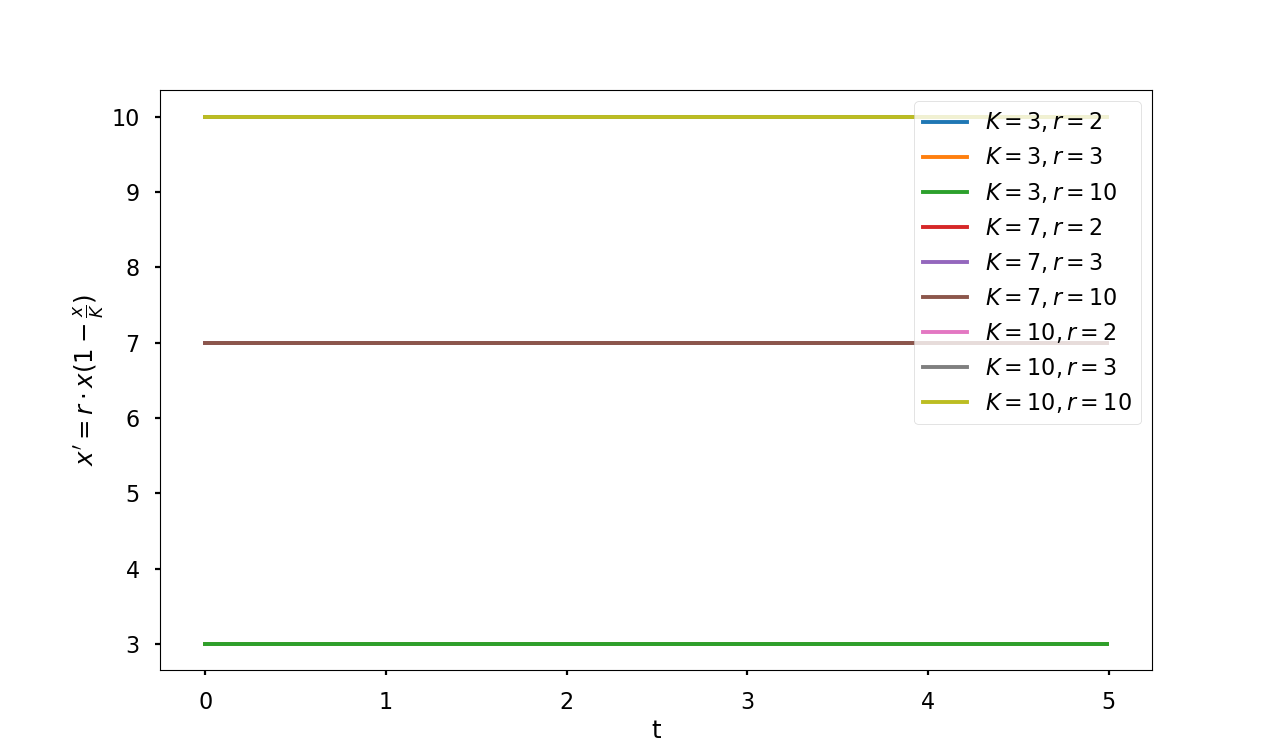
\includegraphics[width=0.8\textwidth]{Figure_1_.png}
  \centering
\end{figure}

Zde je už je vidět, že dané funkce jsou konstantní, proto s velkou
pravděpodobností šlo o chybu.

Jako počáteční hodnotu $x_0$ jsem vybral $x_0 = 0,01$, a to s cílem ukázat,
že na začátku roste funkce jen nepatrně, než přijde "zlom".

\clearpage
\section{Úloha 2}

Pro odvození diferenciální rovnice jsem použil náčrt níže:

\begin{figure}[h]
  \begin{tikzpicture}[scale=2]
    \draw[thick,->, gray] (0,0) -- (4.5,0);
    \draw[thick,->, gray] (0,0) -- (0,3.5);

    \draw[thick]  (1,0) -- (1,2.5) node[below=3cm, left=3pt] {$y_v$};
    \draw[thick] (1,2.5) -- (4,0);
    \draw (1,0) -- (4,0) node[below=7pt, left=2cm] {$x_z - x_v$};

    \draw[very thick] (1,1.25) -- (1,2.5) node[below=1.3cm, left=3pt] {$- y_v'$};
    \draw[very thick] (1,2.5) -- (2.5,1.25) node[above=1.3cm, left=0.7cm] {$v_v$};
    \draw[very thick] (1,1.25) -- (2.5,1.25) node[below=7pt, left=1cm] {$x_v'$};

    \draw[fill=black] (4,0) node[anchor=north west] {zajíc $(x_z, 0)$} circle (0.075);
    \draw[fill=black] (1,2.5) node[anchor=south east] {vlk $(x_v, y_v)$} circle (0.075);

    \draw (1,0) coordinate (A) -- (1,2.5) coordinate (B) -- (4,0) coordinate (C)
      pic [draw, ->, "$\phi$", angle eccentricity=1.5]{angle};
  \end{tikzpicture}
  \centering
\end{figure}

Z tohoto obrázku můžeme odvodit diferenciální rovnici dvěmi způsoby. Buď
vypočítáme úhel $\phi$ a následně za pomoci goniometrických funkcí vypočítáme
změnu, nebo použijeme Pythagorovu větu k získání poměru okamžité rychlosti
vlka $v_v$ ke vzdálenosti.

Jako první mně napadl způsob s použitím goniometrických funkcí. Nejprve
zjistíme úhel $\phi$:

\[
  \phi = \arctan \frac{x_z - x_v}{y_v}
\]

Teď za pomoci jednoduchých úprav získáme změnu jak $x_v'$, tak $y_v'$.
Musíme ale vzít v úvahu, že $y_v$ se celou dobu změnšuje, proto
musíme přidat mínus:

\[
  \sin \phi = \frac{x_v'}{v_v} \ztoho x_v' = v_v \sin\left(\arctan \frac{x_z - x_v}{y_v}\right)
\]
\[
  \cos \phi = \frac{- y_v'}{v_v} \ztoho y_v' = - v_v \cos\left(\arctan \frac{x_z - x_v}{y_v}\right)
\]

Když jsem ale řešil třetí úlohu, přišel jsem na řešení pomocí Pythagorovi
věty, které jsem později upřednostnil z několika důvodů:

\begin{enumerate}
  \item předpokládám, že goniometrické funkce jsou složitější na výpočet
    něž odmocnina 
  \item když se stalo, že $y_v < 0$ (což by se nemělo stávat, ale
    řešil jsem to numericky, tudíž se to mohlo stát, když se vlk
    přiblížil ke zajíci), vlk otočil směr a běžel do nekonečna
    od zajíce. Očekávanější by podle mě bylo, že bude běžet
    rychlostí zajíce dál. A 
  \item bylo praktičtější použít na dvě úlohy stějný způsob
    než dva odlišné způsoby 
\end{enumerate}

Nechť $d_vz$ je vzdálenost vlka od zajíce. Z náčrtku můžeme vidět, že
oba pravoúhlé trojúhelníky jsou si podobné, proto: 
\[
  \frac{x_v'}{x_z - x_v} = \frac{- y_v'}{y_v} = \frac{v_v}{d_{vz}}
\]

Zároveň pomocí Pythagorovi věty můžeme $d_vz$ vypočítat takto:

\[
  d_{vz} = \sqrt{(x_z - x_v)^2 + y_v^2}
\]

Když oba poznatky spojíme, získáme vzorce pro výpočet změn $x_v'$ a $y_v'$:

\[
  x_v' = x_v \cdot \frac{v_v}{\sqrt{(x_z - x_v)^2 + y_v^2}}
\]

\[
  y_v' = - y_v \cdot \frac{v_v}{\sqrt{(x_z - x_v)^2 + y_v^2}}
\]

\clearpage

Výsledný graf vypadá následovně:

\begin{figure}[h]
  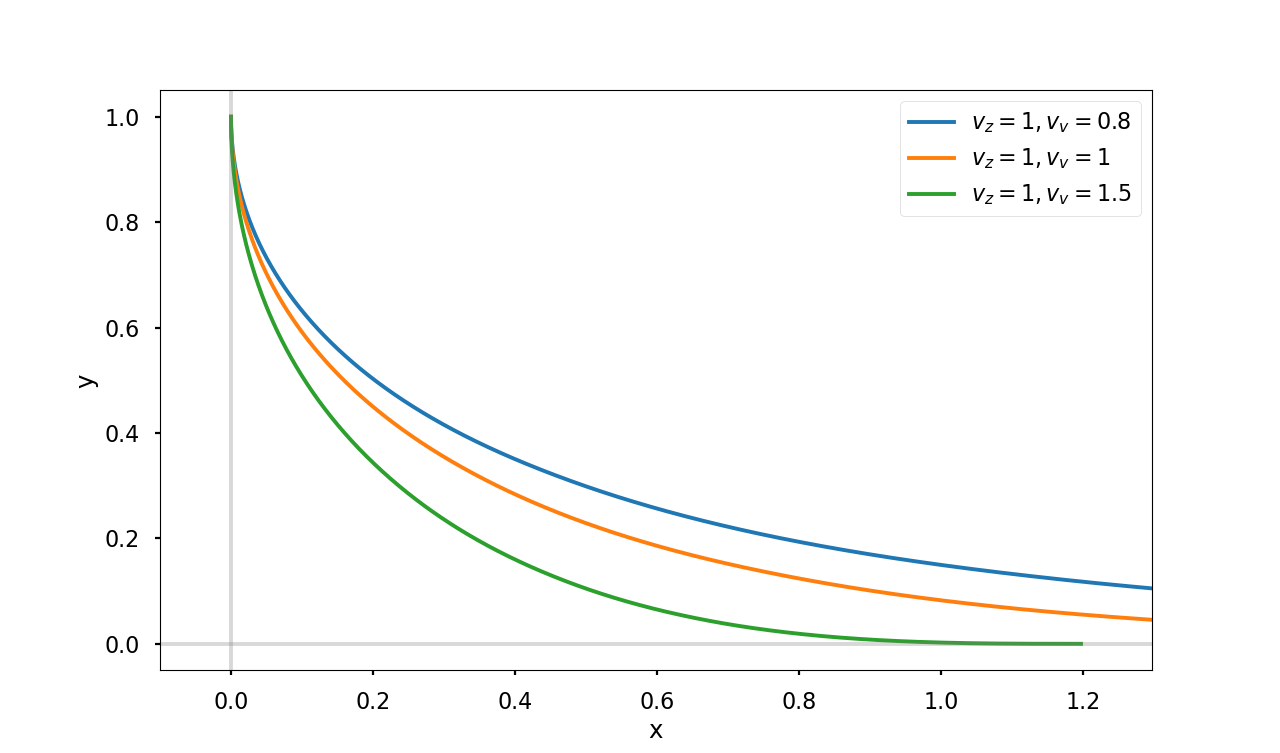
\includegraphics[width=0.8\textwidth]{Figure_2.png}
  \centering
\end{figure}

Pokud bychom chtěli zjistit vzdálenost, kdy vlk chytí zajíce, je potřeba
nastavit, aby se analýza zastavila, když $y_v = 0$ (což při numerickém
řešení lze určit jen přibližně). Pro získání
času konce pak tuto hodnotu vydělíme hodnotou $v_z$. Samozřejmě, pokud bude 
platit $v_v \leq v_z$, nemůžeme tuto hodnotu vypočítat (protože vlk zajíce
nikdy nedohoní).

% Mam analyzovat tvar?

\clearpage
\section{Úloha 3}

V této úloze narozdíl od předchozí budeme nuceni použít postup s
Pythagorovou větou, protože střela se během letu
odchýlý od původního směru o více než $90^{\circ}$, jak uvidíte dále na grafu, 
a hodnotový obor funkce arkustangens je jen $(-90^{\circ}, 90^{\circ})$.

Protože postup získání vzorce je skoro stejný jako v předchozí úloze,
rovnou napíšu výsledný vzorce pro raketu $i \in \{1,2,3\}$:

\[
  x_i' = (x_{i+1} - x_i) \cdot \frac{v}{\sqrt{(x_{i+1} - x_i)^2 + (y_{i+1} - y_i)^2}}
\]
\[
  y_i' = (y_{i+1} - y_i) \cdot \frac{v}{\sqrt{(x_{i+1} - x_i)^2 + (y_{i+1} - y_i)^2}}
\]

A když $i = 4$, pak:

\[
  x_4' = (x_1 - x_4) \cdot \frac{v}{\sqrt{(x_1 - x_4)^2 + (y_1 - y_4)^2}}
\]
\[
  y_4' = (y_1 - y_4) \cdot \frac{v}{\sqrt{(x_1 - x_4)^2 + (y_1 - y_4)^2}}
\]

Výsledný graf je níže:

\begin{figure}[h]
  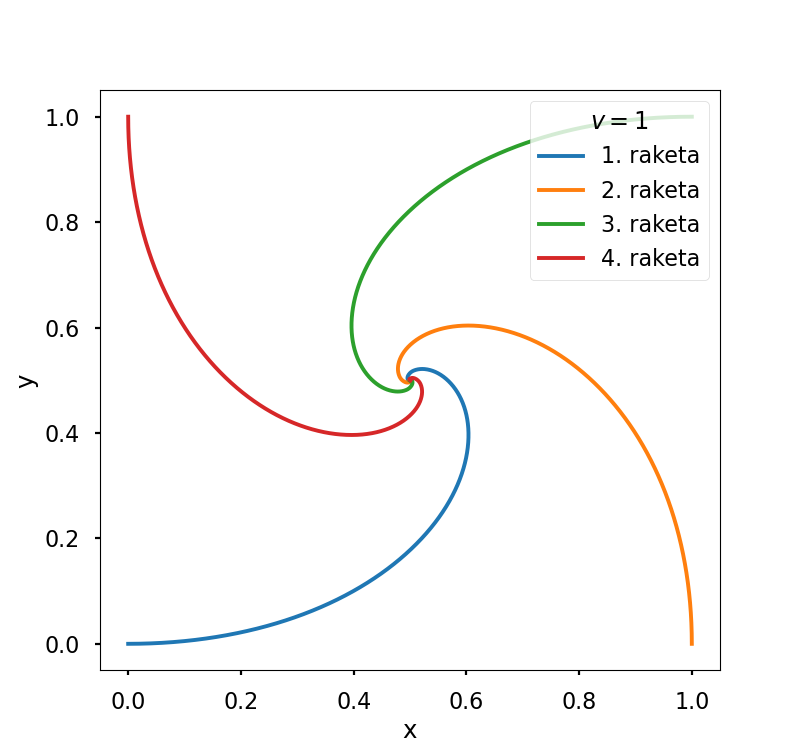
\includegraphics[width=0.7\textwidth]{Figure_3.png}
  \centering
\end{figure}

Výsledná trajektorie se neliší se změnou rychlosti. Rychlost mění jen
čas trvaní letu raket, což dává smysl, když si uvědomíme, že rakety
všechny letí stejnou rychlostí.

\end{document}
